% Ensure that you compile using XeLaTeX !!! PDFTex has problems with some of the packages used
\documentclass[12pt]{article}
\setlength\parindent{0pt}

\usepackage{parskip}
\usepackage[margin=0.5in]{geometry}
\usepackage{fullpage}
\usepackage{moresize}
\usepackage{graphicx}
\usepackage{caption}
\usepackage{subcaption}
\usepackage{float}
\usepackage{xcolor}
\usepackage{soul}
\usepackage{fontspec}
\setmainfont{Doulos SIL}

\begin{document}

\begin{center}
\textbf{{\color{violet}{\HUGE Tuesday, 23 June 2020\\}}}

\textbf{{\color{violet}{\HUGE ALL EXAMS (with notes)\\}}}

\end{center}
\newpage

\begin{center}
\textbf{{\color{blue}{\HUGE START OF EXAM\\}}}

\textbf{{\color{blue}{\HUGE Student ID: 6745\\}}}

\textbf{{\color{blue}{\HUGE 9:30 - 9:50 AM\\}}}

\end{center}
\newpage

{\large Question 1}\\

Source: Day 9 Handout, Question 1\\

Explain why the concept of an alternation either is or is not useful for understanding this dataset.\\

\begin{figure}[H]
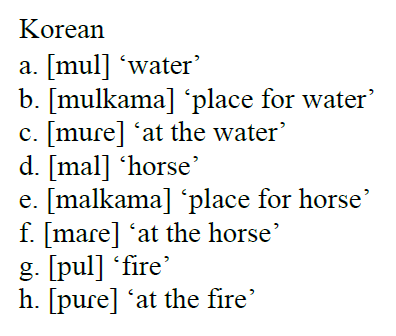
\includegraphics{../images/korean.png}
\end{figure}

~\\
INSTRUCTOR NOTES: is useful -- root morphemes alternate, so we can decide which sounds we need to analyze


\vfill
Excellent (3) ~~~ Good (2.2) ~~~ Fair (1.7) ~~~ Poor (0)
\newpage

{\large Question 2}\\

Source: Day 10 Discussion\\

Explain what the given feature’s value is for this class of sounds, and why.\\

{[approximant]}

nasals


~\\
INSTRUCTOR NOTES: [-], because air can't escape through the mouth ([+approx] sounds have a narrowing in the vocal tract, but air escapes without friction)


\vfill
Excellent (3) ~~~ Good (2.2) ~~~ Fair (1.7) ~~~ Poor (0)
\newpage

{\large Question 3}\\

Source: Final Exam Dataset\\

Explain what the underlying representation of these morphemes would be and why.\\

`mix', `past'

\begin{figure}[H]
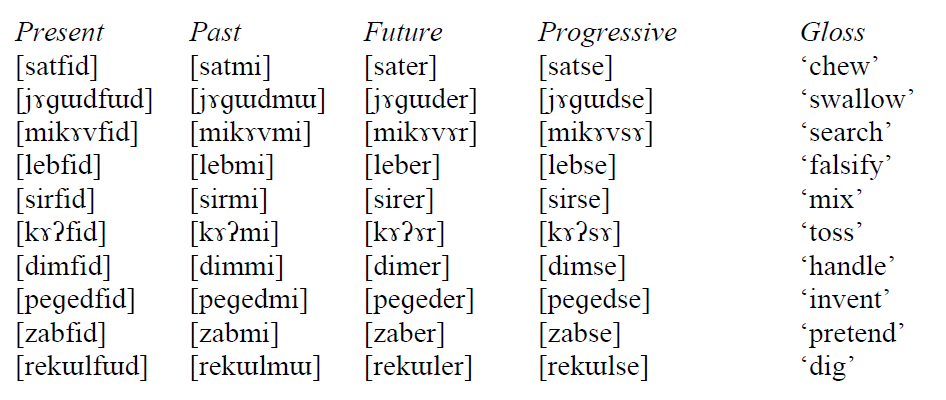
\includegraphics{../images/final_dataset.png}
\end{figure}

~\\
INSTRUCTOR NOTES: For any morpheme that doesn’t alternate, its UR should be the same as its SR.  For the morphemes that alternate, the back-vowel version occurs in the narrower set of contexts (after a back vowel of the same height), so should be the one that we write a rule for. The front-vowel version occurs in the wider / elsewhere set of contexts (after a front vowel and after a back vowel of a different height), so this should be the UR. So in this case, we have the non-alternating root morpheme ‘mix’ /sir/ and the alternating suffix morpheme 'past' /mi/.


\vfill
Excellent (3) ~~~ Good (2.2) ~~~ Fair (1.7) ~~~ Poor (0)
\newpage

{\large Question 4}\\

Source: Day 11 Handout, Question 5\\

Explain why this template either does or does not allow syllables of this type to occur.\\

V

\begin{figure}[H]
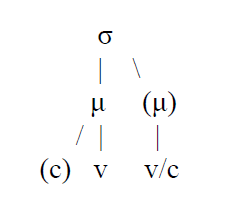
\includegraphics{../images/ponapean_syllabletemplate.png}
\end{figure}

~\\
INSTRUCTOR NOTES: allowed


\vfill
Excellent (3) ~~~ Good (2.2) ~~~ Fair (1.7) ~~~ Poor (0)
\newpage

{\large Question 5}\\

Source: Day 8 Handout, Question 7\\

Explain why each numbered, underlined statement is true or false. If it is false, explain one way that you could correct it.\\

Sound is an invisible phenomenon. Sound can travel through any substance, $^1$\ul{such as a liquid, solid, or a gas.} $^2$\ul{It involves the transfer of the matter in that substance} from one place to another.\\\\Sound is a particular kind of wave known as $^3$\ul{a compression wave}. $^4$\ul{When the molecules are really close together, we say they are ``rarefied'' and when they are really far apart, we say they are ``compressed.''}


~\\
INSTRUCTOR NOTES: 1 - true.\\2 - false (it involves the transfer of energy... or anything about the matter itself not moving but only vibrating, etc). \\3 - true.\\4 - false (when the molecules are really close together, we say they are compressed and when the molecules are really far apart, we say they are rarefied).


\vfill
Excellent (3) ~~~ Good (2.2) ~~~ Fair (1.7) ~~~ Poor (0)
\newpage

{\large Question 6}\\

Source: Day 12 Handout, Question 7\\

Explain how you would figure out the tone-mapping procedures that apply in this dataset.\\

\begin{figure}[H]
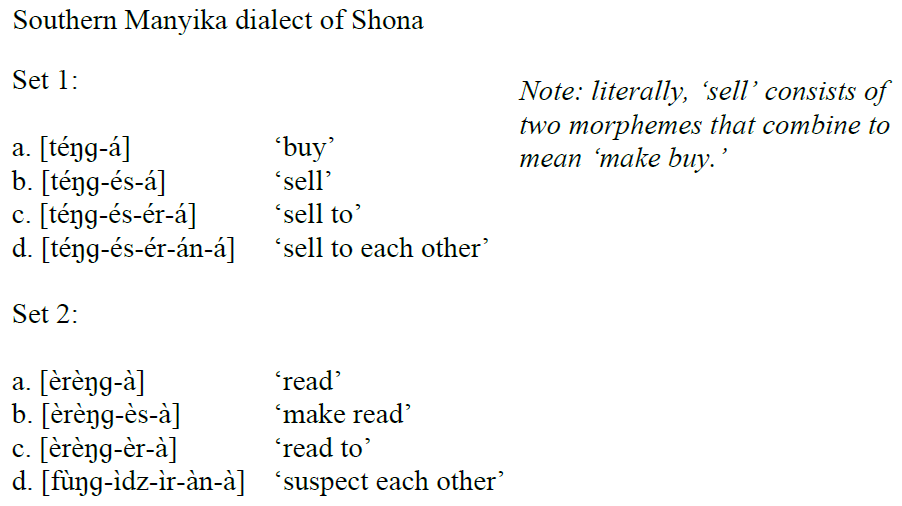
\includegraphics{../images/shona.png}
\end{figure}

~\\
INSTRUCTOR NOTES: You probably start with procedures that you know work for some other language like Mende, and see whether they work here; in this case, there's only one underlying tone in each word, and it gets linked to every TBU, so you probably just need something like initial linking and then Leftover-TBU linking (there will never be any leftover tones)


\vfill
Excellent (3) ~~~ Good (2.2) ~~~ Fair (1.7) ~~~ Poor (0)
\newpage

\begin{center}
\textbf{{\color{red}{\HUGE END OF EXAM}}}\\

\end{center}
\newpage

\begin{center}
\textbf{{\color{blue}{\HUGE START OF EXAM\\}}}

\textbf{{\color{blue}{\HUGE Student ID: 6427\\}}}

\textbf{{\color{blue}{\HUGE 9:50 - 10:10 AM\\}}}

\end{center}
\newpage

{\large Question 1}\\

Source: Day 9 Handout, Question 1\\

Explain why the concept of an alternation either is or is not useful for understanding this dataset.\\

\begin{figure}[H]
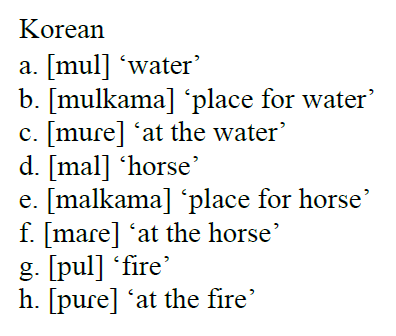
\includegraphics{../images/korean.png}
\end{figure}

~\\
INSTRUCTOR NOTES: is useful -- root morphemes alternate, so we can decide which sounds we need to analyze


\vfill
Excellent (3) ~~~ Good (2.2) ~~~ Fair (1.7) ~~~ Poor (0)
\newpage

{\large Question 2}\\

Source: Final Exam Dataset\\

Explain how you would go about figuring out what to analyse in this dataset.\\

\begin{figure}[H]
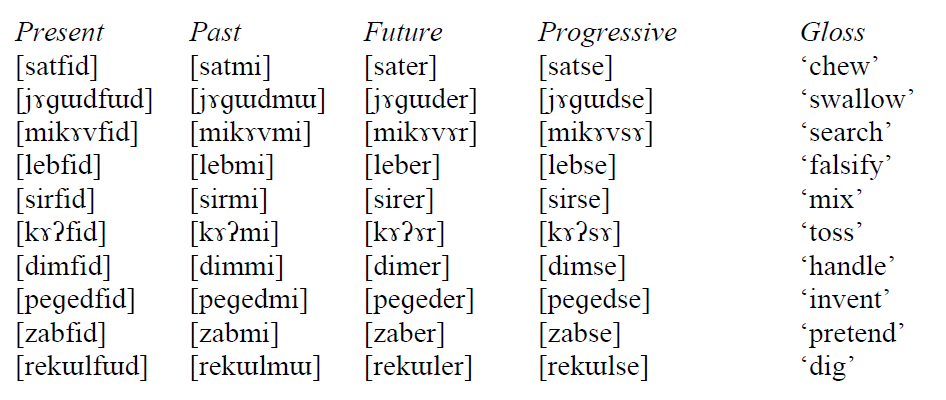
\includegraphics{../images/final_dataset.png}
\end{figure}

~\\
INSTRUCTOR NOTES: The first thing to do is a morphological analysis. There should be morphemes that represent each of the four tenses / aspects (present, past, future, and progressive), and morphemes that represent each root. The morphemes representing the tenses appear as (relatively) consistent forms in the columns; the morphemes representing the roots appear as consistent forms in the rows. Doing this reveals that the final 3 segments in the present forms and the final two segments in the progressive forms are suffixes (there are no zero morphemes, and all components have a one-to-one correspondence). Then we check for alternations. The alternations here are in the suffixes; each of the four suffixes has two forms. There are therefore four alternations, with two allomorphs each. So, what we need to analyze are the alternations in the suffix forms, where we see vowels alternating. Two of the alternations involve [i] and [ɯ], and the other two alternations involve [e] and [ɤ]. In each case, there’s a front vowel and a back vowel, which are otherwise matched for height and rounding, so we can likely generalize across the alternations.


\vfill
Excellent (3) ~~~ Good (2.2) ~~~ Fair (1.7) ~~~ Poor (0)
\newpage

{\large Question 3}\\

Source: Day 11 Handout, Question 8\\

Explain how you could modify the rule-based approach to take into account the sonority sequencing principle.\\

\begin{figure}[H]
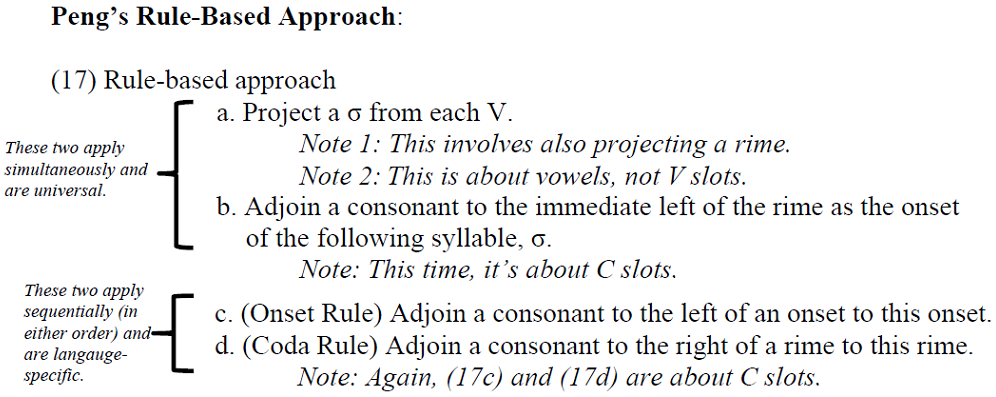
\includegraphics{../images/peng_rules.png}
\end{figure}

~\\
INSTRUCTOR NOTES: basically, you need to say something like: Modified onset rule: adjoin a consonant to the left of an onset to that onset, if the consonant has a LOWER sonority than the onset


\vfill
Excellent (3) ~~~ Good (2.2) ~~~ Fair (1.7) ~~~ Poor (0)
\newpage

{\large Question 4}\\

Source: Day 10 Discussion\\

Explain what the given feature’s value is for this class of sounds, and why.\\

{[LABIAL]}

interdentals


~\\
INSTRUCTOR NOTES: 0, because interdentals aren't [LABIAL], but [LABIAL] is monovalent, so they're not [-labial]


\vfill
Excellent (3) ~~~ Good (2.2) ~~~ Fair (1.7) ~~~ Poor (0)
\newpage

{\large Question 5}\\

Source: Day 8 Handout, Question 3\\

Explain what you see in the spectrogram that tells you about the properties of the sounds in the pictured word.\\

\begin{figure}[H]
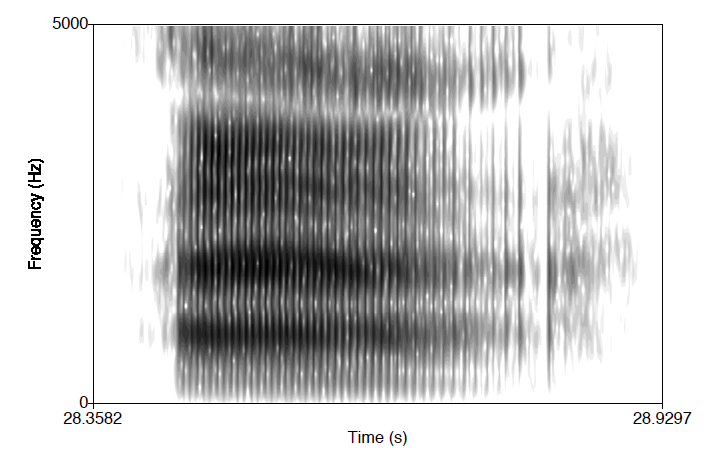
\includegraphics{../images/spectrogram_aaah.png}
\end{figure}

~\\
INSTRUCTOR NOTES: aaah: just a vowel; formants are very steady; F1 and F2 are pretty close to each other; F1 somewhat high and F2 somewhat low


\vfill
Excellent (3) ~~~ Good (2.2) ~~~ Fair (1.7) ~~~ Poor (0)
\newpage

{\large Question 6}\\

Source: Quiz 10, Question 3\\

Section 4.2 of chapter 13 in the Peng textbook presented an autosegmental analysis of Mende tone distribution. Explain why the form shown below should NOT be the UR for any morpheme in Mende.\\

\begin{figure}[H]
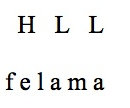
\includegraphics{../images/mende_junction_b.png}
\end{figure}

~\\
INSTRUCTOR NOTES: There's no reason to violate the OCP in the UR of a single morpheme, but this one has two adjacent L tones


\vfill
Excellent (3) ~~~ Good (2.2) ~~~ Fair (1.7) ~~~ Poor (0)
\newpage

\begin{center}
\textbf{{\color{red}{\HUGE END OF EXAM}}}\\

\end{center}
\newpage

\begin{center}
\textbf{{\color{blue}{\HUGE START OF EXAM\\}}}

\textbf{{\color{blue}{\HUGE Student ID: 3773\\}}}

\textbf{{\color{blue}{\HUGE 10:10 - 10:30 AM\\}}}

\end{center}
\newpage

{\large Question 1}\\

Source: Day 11 Handout, Question 12\\

Explain how understanding syllable structure helps understand the motivation for the process(es) seen in this data.\\

\begin{figure}[H]
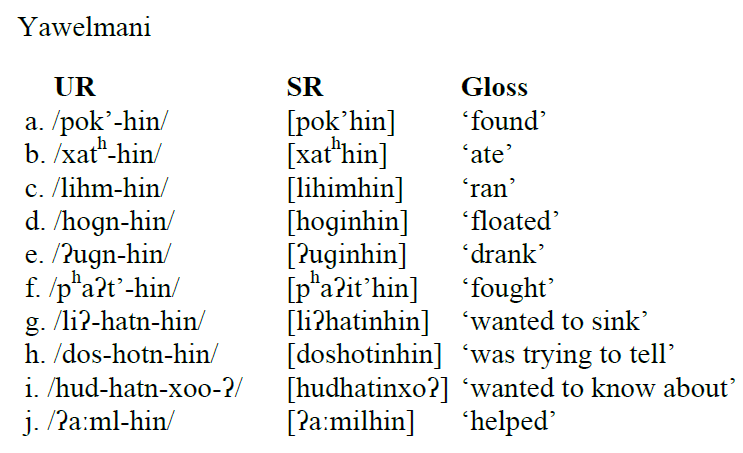
\includegraphics{../images/yawelmani.png}
\end{figure}

~\\
INSTRUCTOR NOTES: although syllabification must happen after insertion, the insertion is motivated by making things syllabifiable -- we insert a vowel into a sequence of CCC in order to prevent any complex onsets / codas or syllabic consonants from having to be used


\vfill
Excellent (3) ~~~ Good (2.2) ~~~ Fair (1.7) ~~~ Poor (0)
\newpage

{\large Question 2}\\

Source: Final Exam Dataset\\

Explain what the underlying representation of these morphemes would be and why.\\

`dig', `future'

\begin{figure}[H]
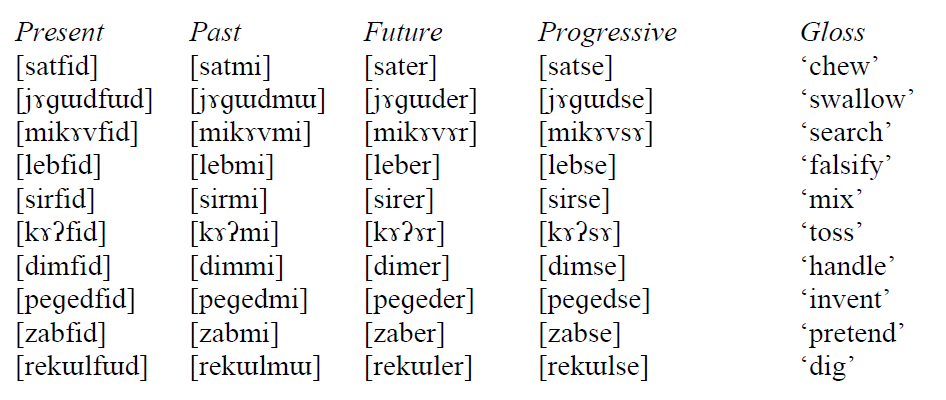
\includegraphics{../images/final_dataset.png}
\end{figure}

~\\
INSTRUCTOR NOTES: For any morpheme that doesn’t alternate, its UR should be the same as its SR.  For the morphemes that alternate, the back-vowel version occurs in the narrower set of contexts (after a back vowel of the same height), so should be the one that we write a rule for. The front-vowel version occurs in the wider / elsewhere set of contexts (after a front vowel and after a back vowel of a different height), so this should be the UR. So in this case, we have the non-alternating root morpheme ‘dig’ /rekɯl/ and the alternating suffix morpheme 'future' /er/.


\vfill
Excellent (3) ~~~ Good (2.2) ~~~ Fair (1.7) ~~~ Poor (0)
\newpage

{\large Question 3}\\

Source: Day 8 Handout, Question 1\\

Explain what (if anything) the letter below represents on this waveform.\\

A

\begin{figure}[H]
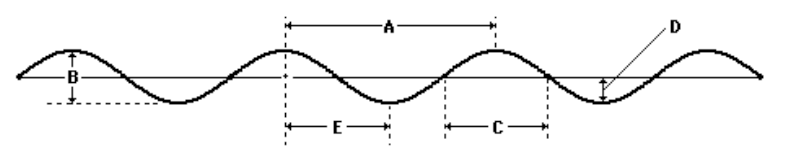
\includegraphics{../images/sinusoid.png}
\end{figure}

~\\
INSTRUCTOR NOTES: wavelength or period


\vfill
Excellent (3) ~~~ Good (2.2) ~~~ Fair (1.7) ~~~ Poor (0)
\newpage

{\large Question 4}\\

Source: Day 10 Handout, Question 6 (Homework 4, Question 2)\\

Explain how you should use phonological features in this rule. Which parts of the rule should include features, and what features might they be? You don't have to give an exact set of features, but what kinds of features would be involved?\\

/n/ → ∅ / {[m]} \_\_ \#

\begin{figure}[H]
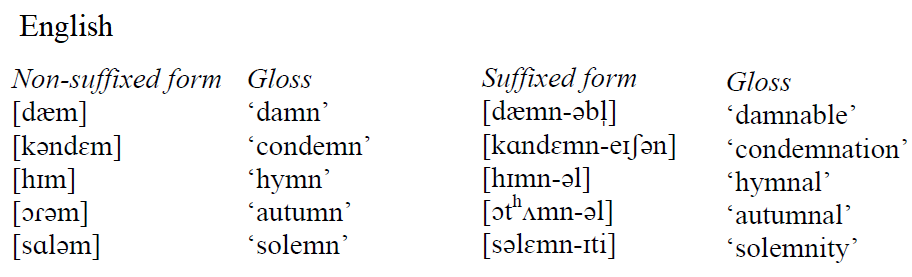
\includegraphics{../images/english_stemalternations.png}
\end{figure}

~\\
INSTRUCTOR NOTES: you really can't use features for any of this, because it's all individual segments


\vfill
Excellent (3) ~~~ Good (2.2) ~~~ Fair (1.7) ~~~ Poor (0)
\newpage

{\large Question 5}\\

Source: Day 9 Handout, Question 4\\

Explain which morpheme(s) in this dataset alternate and how that helps you do a phonological analysis.\\

\begin{figure}[H]
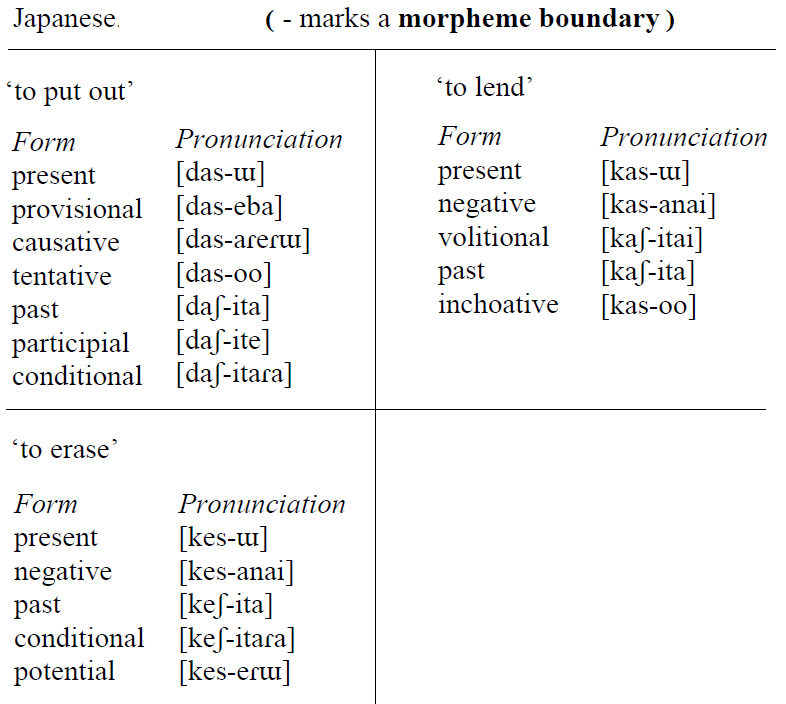
\includegraphics{../images/japanese_verbs.png}
\end{figure}

~\\
INSTRUCTOR NOTES: each verb root alternates, so we know the sounds we need to analyze are the predictable occurrence of [s] and [ʃ]


\vfill
Excellent (3) ~~~ Good (2.2) ~~~ Fair (1.7) ~~~ Poor (0)
\newpage

{\large Question 6}\\

Source: Day 12 Handout, Question 6\\

Explain how you would figure out the tone-mapping procedures that apply in this dataset.\\

\begin{figure}[H]
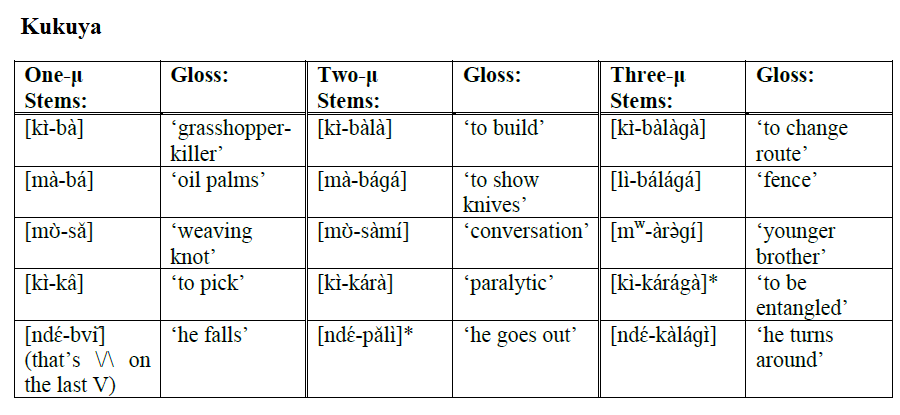
\includegraphics{../images/kukuya.png}
\end{figure}

~\\
INSTRUCTOR NOTES: You probably start with procedures that you know work for some other language like Mende, and see whether they work here. In this case, we (1) look at cases of words that have one of the contour tones, because words with only H or only L will just always have a single tone associated with all of the TBUs, but contour tones can help you see e.g. “where” the contour happens; (2) look at cases of words with a mismatch in the number of tones and TBUs (e.g. HL tones and VVV, or LHL tones and VV), because these are cases where one-to-one mapping will fail. By seeing that the “tail” of contours is to the left, not the right (e.g., it’s LLH not LHH) and that in the triple-tone words with two TBUs, we have the contour to the left (LH, then L; not L, then HL), we see that the “leftover” stuff needs to be on the left edge instead of the right edge. Hence, the initial mapping procedure should proceed from right to left instead of left to right.


\vfill
Excellent (3) ~~~ Good (2.2) ~~~ Fair (1.7) ~~~ Poor (0)
\newpage

\begin{center}
\textbf{{\color{red}{\HUGE END OF EXAM}}}\\

\end{center}
\newpage

\begin{center}
\textbf{{\color{blue}{\HUGE START OF EXAM\\}}}

\textbf{{\color{blue}{\HUGE Student ID: 9303\\}}}

\textbf{{\color{blue}{\HUGE 10:30 - 10:50 AM\\}}}

\end{center}
\newpage

{\large Question 1}\\

Source: Day 11 Handout, Question 5\\

Explain why this template either does or does not allow syllables of this type to occur.\\

V

\begin{figure}[H]
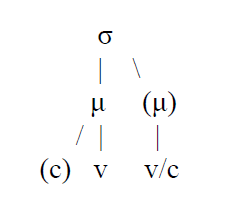
\includegraphics{../images/ponapean_syllabletemplate.png}
\end{figure}

~\\
INSTRUCTOR NOTES: allowed


\vfill
Excellent (3) ~~~ Good (2.2) ~~~ Fair (1.7) ~~~ Poor (0)
\newpage

{\large Question 2}\\

Source: Final Exam Dataset\\

Explain what the underlying representation of these morphemes would be and why.\\

`dig', `future'

\begin{figure}[H]
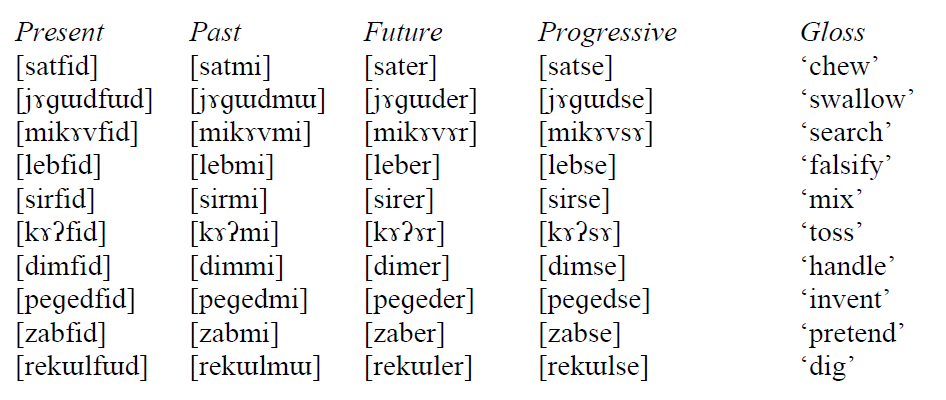
\includegraphics{../images/final_dataset.png}
\end{figure}

~\\
INSTRUCTOR NOTES: For any morpheme that doesn’t alternate, its UR should be the same as its SR.  For the morphemes that alternate, the back-vowel version occurs in the narrower set of contexts (after a back vowel of the same height), so should be the one that we write a rule for. The front-vowel version occurs in the wider / elsewhere set of contexts (after a front vowel and after a back vowel of a different height), so this should be the UR. So in this case, we have the non-alternating root morpheme ‘dig’ /rekɯl/ and the alternating suffix morpheme 'future' /er/.


\vfill
Excellent (3) ~~~ Good (2.2) ~~~ Fair (1.7) ~~~ Poor (0)
\newpage

{\large Question 3}\\

Source: Day 10 Handout, Question 6 (Day 7 Handout, Question 7)\\

Explain how you should use phonological features to combine these rules.\\

/s/ → {[ʃ]} / \_\_ {[i]} \\/z/ → {[dʒ]} / \_\_ {[i]}

\begin{figure}[H]
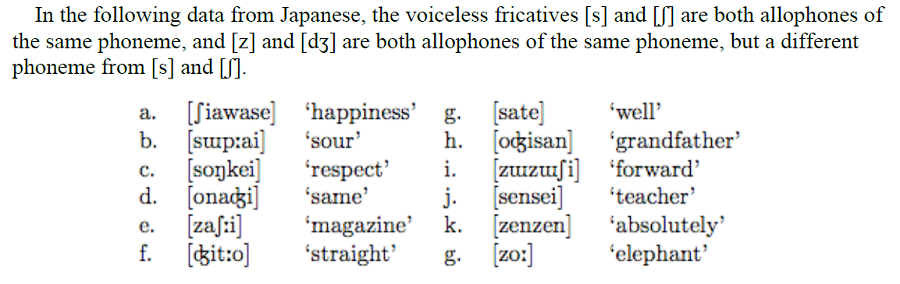
\includegraphics{../images/japanese.png}
\end{figure}

~\\
INSTRUCTOR NOTES: input should be alveolar fricatives, output should be just a change in place of articulation; context is still [i]; something like [CORONAL, +strid] --> [-ant, +dist] / \_\_ [i]; note that this won't directly account for why the voiced one becomes an affricate


\vfill
Excellent (3) ~~~ Good (2.2) ~~~ Fair (1.7) ~~~ Poor (0)
\newpage

{\large Question 4}\\

Source: Day 9 Handout, Question 4\\

Explain which morpheme(s) in this dataset alternate and how that helps you do a phonological analysis.\\

\begin{figure}[H]
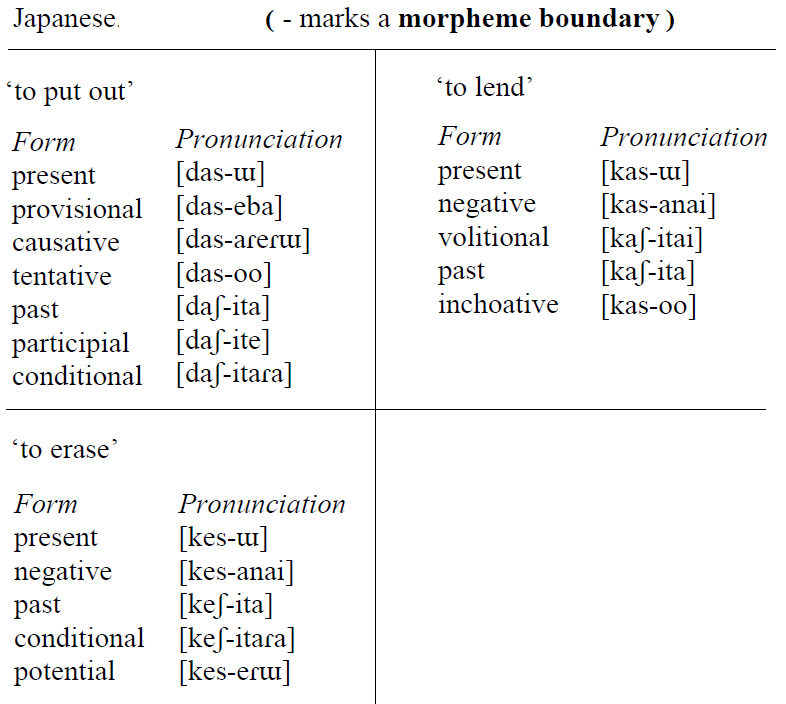
\includegraphics{../images/japanese_verbs.png}
\end{figure}

~\\
INSTRUCTOR NOTES: each verb root alternates, so we know the sounds we need to analyze are the predictable occurrence of [s] and [ʃ]


\vfill
Excellent (3) ~~~ Good (2.2) ~~~ Fair (1.7) ~~~ Poor (0)
\newpage

{\large Question 5}\\

Source: Day 8 Handout, Question 1\\

Explain what (if anything) the letter below represents on this waveform.\\

B

\begin{figure}[H]
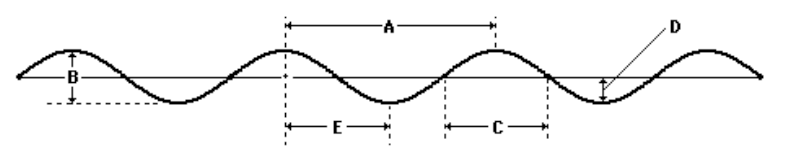
\includegraphics{../images/sinusoid.png}
\end{figure}

~\\
INSTRUCTOR NOTES: nothing (twice amplitude)


\vfill
Excellent (3) ~~~ Good (2.2) ~~~ Fair (1.7) ~~~ Poor (0)
\newpage

{\large Question 6}\\

Source: Day 12 Handout, Question 5\\

Explain which of the three rules will apply to the form given below, and whether each of those rules would have an effect or not.\\

Peng’s Tone-Mapping Procedure for Mende: \begin{enumerate} \item L-to-R association: Associate the first tone to the first TBU, the second tone to the second TBU, and so on, until all tones or all TBUS are exhausted. \item Last-TBU Linking: Associate any remaining unlinked tones to the last TBU. \item Last-Tone Linking: Associate the last tone to any TBU without a tone. \end{enumerate}

\begin{figure}[H]
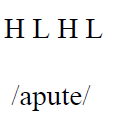
\includegraphics{../images/mendetone_d.png}
\end{figure}

~\\
INSTRUCTOR NOTES: L-to-R association applies, and links the first three tones (H L H) to the first three TBUs ([a], [u], [e]). Then last-TBU linking applies and links the leftover L tone to the last TBU ([e]). Last-tone linking will not apply because there are no leftover TBUs.


\vfill
Excellent (3) ~~~ Good (2.2) ~~~ Fair (1.7) ~~~ Poor (0)
\newpage

\begin{center}
\textbf{{\color{red}{\HUGE END OF EXAM}}}\\

\end{center}
\newpage

\begin{center}
\textbf{{\color{blue}{\HUGE START OF EXAM\\}}}

\textbf{{\color{blue}{\HUGE Student ID: 5824\\}}}

\textbf{{\color{blue}{\HUGE 10:50 - 11:10 AM\\}}}

\end{center}
\newpage

{\large Question 1}\\

Source: Day 11 Handout, Question 5\\

Explain why this template either does or does not allow syllables of this type to occur.\\

CVVC

\begin{figure}[H]
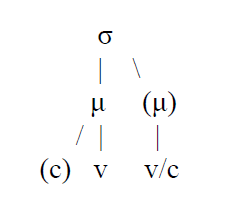
\includegraphics{../images/ponapean_syllabletemplate.png}
\end{figure}

~\\
INSTRUCTOR NOTES: not allowed


\vfill
Excellent (3) ~~~ Good (2.2) ~~~ Fair (1.7) ~~~ Poor (0)
\newpage

{\large Question 2}\\

Source: Final Exam Dataset\\

Explain what the basic phonological analysis of this dataset is, and what the key pieces of evidence are.\\

\begin{figure}[H]
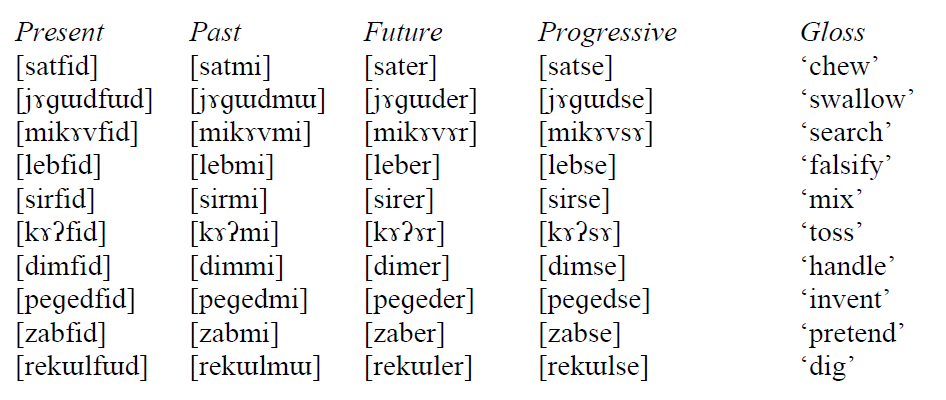
\includegraphics{../images/final_dataset.png}
\end{figure}

~\\
INSTRUCTOR NOTES: The basic analysis here is that vowels of the same height need to agree in terms of backness. We see this in suffix alternations: there are four alternating suffixes, each with a back and front variant, and two of them have high vowels while two of them have mid vowels. Whenever the suffix comes after a root containing a back vowel at the same height as the suffix, the suffix also contains a back vowel, but when the root contains either a front vowel or a back vowel at a different height, the suffix contains the front vowel. Thus, we posit the front versions as the URs of the suffixes, because they occur in the wider set of contexts, and write a rule of vowel backing that only applies when the target vowel follows a back context vowel of the same height.


\vfill
Excellent (3) ~~~ Good (2.2) ~~~ Fair (1.7) ~~~ Poor (0)
\newpage

{\large Question 3}\\

Source: Day 10 Discussion\\

Explain why the given feature's value varies across this set of sounds.\\

{[voice]}

glottalized obstruents


~\\
INSTRUCTOR NOTES: includes both voiced and voiceless glottalized obstruents -- obs. can themselves be voiced or voiceless


\vfill
Excellent (3) ~~~ Good (2.2) ~~~ Fair (1.7) ~~~ Poor (0)
\newpage

{\large Question 4}\\

Source: Day 12 Handout, Question 5\\

Explain which of the three rules will apply to the form given below, and whether each of those rules would have an effect or not.\\

Peng’s Tone-Mapping Procedure for Mende: \begin{enumerate} \item L-to-R association: Associate the first tone to the first TBU, the second tone to the second TBU, and so on, until all tones or all TBUS are exhausted. \item Last-TBU Linking: Associate any remaining unlinked tones to the last TBU. \item Last-Tone Linking: Associate the last tone to any TBU without a tone. \end{enumerate}

\begin{figure}[H]
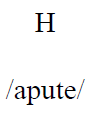
\includegraphics{../images/mendetone_b.png}
\end{figure}

~\\
INSTRUCTOR NOTES: L-to-R association applies and links the H tone to the first TBU [a]; last-TBU linking doesn't apply because there are no leftover tones; then last-tone linking does apply, and connects all of the leftover TBUs (in this case, [u] and [e]) to the final tone (in this case, H)


\vfill
Excellent (3) ~~~ Good (2.2) ~~~ Fair (1.7) ~~~ Poor (0)
\newpage

{\large Question 5}\\

Source: Day 8 Handout, Question 3\\

Explain what you see in the spectrogram that tells you about the properties of the sounds in the pictured word.\\

\begin{figure}[H]
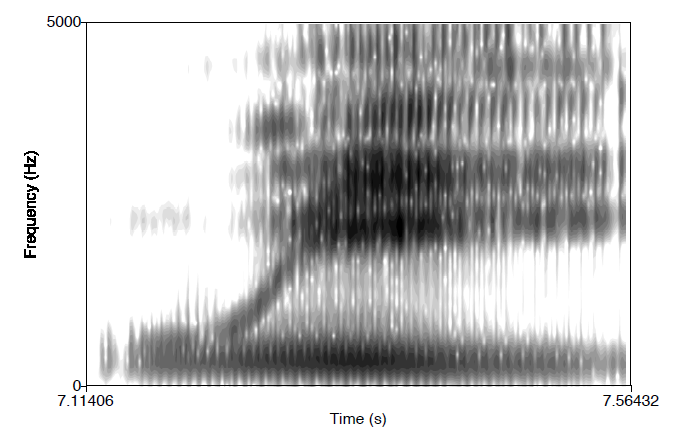
\includegraphics{../images/spectrogram_we.png}
\end{figure}

~\\
INSTRUCTOR NOTES: we: starts paler, then darker, so glide plus vowel; F1 pretty constantly low (=high V); F2 starts very low and then swoops up (=starts back and goes front)


\vfill
Excellent (3) ~~~ Good (2.2) ~~~ Fair (1.7) ~~~ Poor (0)
\newpage

{\large Question 6}\\

Source: Day 9 Handout, Question 3\\

Explain which morpheme(s) in this dataset alternate and how that helps you do a phonological analysis.\\

\begin{figure}[H]
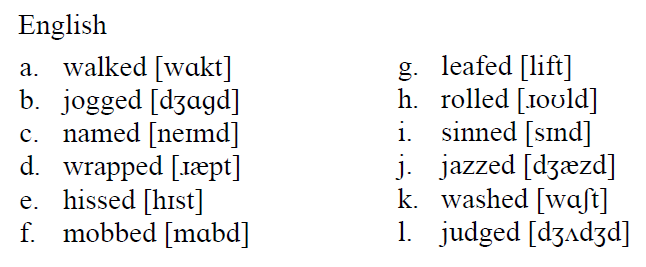
\includegraphics{../images/english_past.png}
\end{figure}

~\\
INSTRUCTOR NOTES: the past tense morpheme alternates, so we know we need to analyze the predictable occurrence of [t] vs. [d]


\vfill
Excellent (3) ~~~ Good (2.2) ~~~ Fair (1.7) ~~~ Poor (0)
\newpage

\begin{center}
\textbf{{\color{red}{\HUGE END OF EXAM}}}\\

\end{center}
\newpage

\begin{center}
\textbf{{\color{blue}{\HUGE START OF EXAM\\}}}

\textbf{{\color{blue}{\HUGE Student ID: 5540\\}}}

\textbf{{\color{blue}{\HUGE 11:10 - 11:30 AM\\}}}

\end{center}
\newpage

{\large Question 1}\\

Source: Day 11 Handout, Question 13\\

Explain how understanding syllable structure helps understand the motivation for the process(es) seen in this data.\\

\begin{figure}[H]
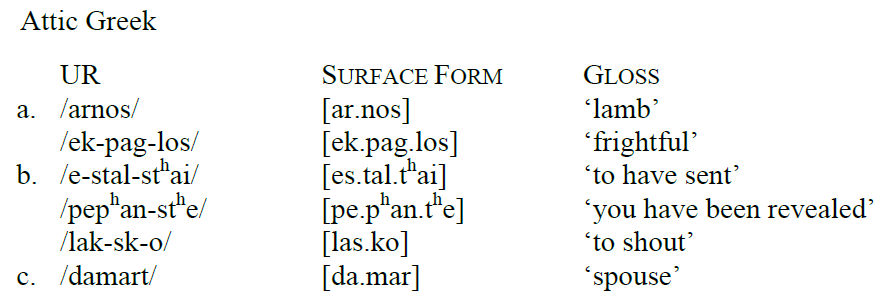
\includegraphics{../images/atticgreek.png}
\end{figure}

~\\
INSTRUCTOR NOTES: although syllabification must happen after deletion, the deletion is motivated by making things syllabifiable -- we delete a consonant from a sequence of CCC in order to prevent any complex onsets / codas or syllabic consonants from having to be used


\vfill
Excellent (3) ~~~ Good (2.2) ~~~ Fair (1.7) ~~~ Poor (0)
\newpage

{\large Question 2}\\

Source: Final Exam Dataset\\

Explain what the underlying representation of these morphemes would be and why.\\

`mix', `past'

\begin{figure}[H]
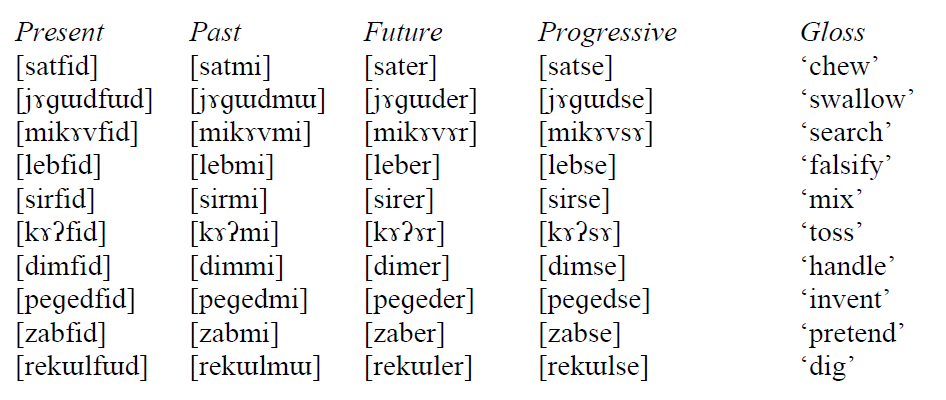
\includegraphics{../images/final_dataset.png}
\end{figure}

~\\
INSTRUCTOR NOTES: For any morpheme that doesn’t alternate, its UR should be the same as its SR.  For the morphemes that alternate, the back-vowel version occurs in the narrower set of contexts (after a back vowel of the same height), so should be the one that we write a rule for. The front-vowel version occurs in the wider / elsewhere set of contexts (after a front vowel and after a back vowel of a different height), so this should be the UR. So in this case, we have the non-alternating root morpheme ‘mix’ /sir/ and the alternating suffix morpheme 'past' /mi/.


\vfill
Excellent (3) ~~~ Good (2.2) ~~~ Fair (1.7) ~~~ Poor (0)
\newpage

{\large Question 3}\\

Source: Day 8 Handout, Question 3\\

Explain what you see in the spectrogram that tells you about the properties of the sounds in the pictured word.\\

\begin{figure}[H]
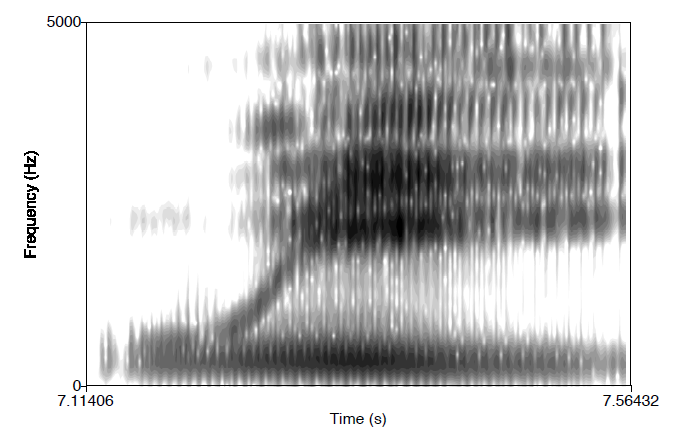
\includegraphics{../images/spectrogram_we.png}
\end{figure}

~\\
INSTRUCTOR NOTES: we: starts paler, then darker, so glide plus vowel; F1 pretty constantly low (=high V); F2 starts very low and then swoops up (=starts back and goes front)


\vfill
Excellent (3) ~~~ Good (2.2) ~~~ Fair (1.7) ~~~ Poor (0)
\newpage

{\large Question 4}\\

Source: Day 12 Handout, Question 6\\

Explain how you would figure out the tone-mapping procedures that apply in this dataset.\\

\begin{figure}[H]
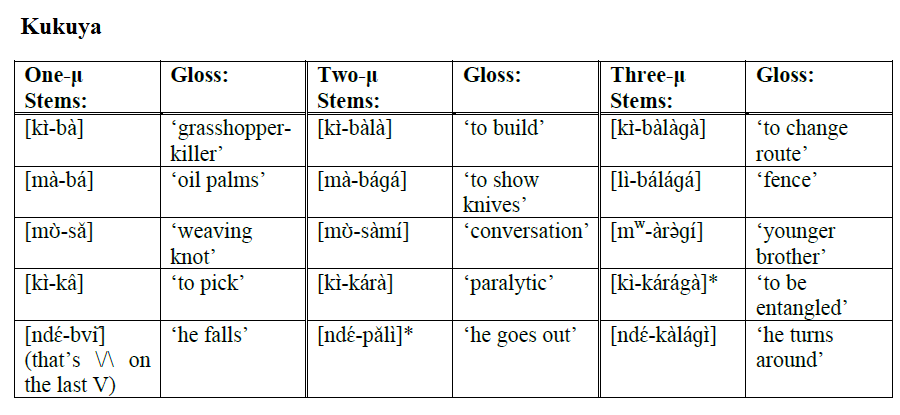
\includegraphics{../images/kukuya.png}
\end{figure}

~\\
INSTRUCTOR NOTES: You probably start with procedures that you know work for some other language like Mende, and see whether they work here. In this case, we (1) look at cases of words that have one of the contour tones, because words with only H or only L will just always have a single tone associated with all of the TBUs, but contour tones can help you see e.g. “where” the contour happens; (2) look at cases of words with a mismatch in the number of tones and TBUs (e.g. HL tones and VVV, or LHL tones and VV), because these are cases where one-to-one mapping will fail. By seeing that the “tail” of contours is to the left, not the right (e.g., it’s LLH not LHH) and that in the triple-tone words with two TBUs, we have the contour to the left (LH, then L; not L, then HL), we see that the “leftover” stuff needs to be on the left edge instead of the right edge. Hence, the initial mapping procedure should proceed from right to left instead of left to right.


\vfill
Excellent (3) ~~~ Good (2.2) ~~~ Fair (1.7) ~~~ Poor (0)
\newpage

{\large Question 5}\\

Source: Quiz 8, Question 3\\

Explain why this featural specification either does or does not match the given sound.\\

{[+consonantal]}, {[+sonorant]}

{[m]}


~\\
INSTRUCTOR NOTES: matches


\vfill
Excellent (3) ~~~ Good (2.2) ~~~ Fair (1.7) ~~~ Poor (0)
\newpage

{\large Question 6}\\

Source: Day 9 Handout, Question 3\\

Explain which morpheme(s) in this dataset alternate and how that helps you do a phonological analysis.\\

\begin{figure}[H]
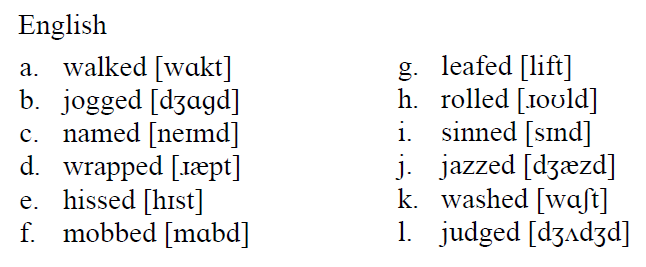
\includegraphics{../images/english_past.png}
\end{figure}

~\\
INSTRUCTOR NOTES: the past tense morpheme alternates, so we know we need to analyze the predictable occurrence of [t] vs. [d]


\vfill
Excellent (3) ~~~ Good (2.2) ~~~ Fair (1.7) ~~~ Poor (0)
\newpage

\begin{center}
\textbf{{\color{red}{\HUGE END OF EXAM}}}\\

\end{center}
\newpage

\begin{center}
\textbf{{\color{blue}{\HUGE START OF EXAM\\}}}

\textbf{{\color{blue}{\HUGE Student ID: 1887\\}}}

\textbf{{\color{blue}{\HUGE 11:30 - 11:50 AM\\}}}

\end{center}
\newpage

{\large Question 1}\\

Source: Day 9 Handout, Question 2\\

Explain why the concept of an alternation either is or is not useful for understanding this dataset.\\

\begin{figure}[H]
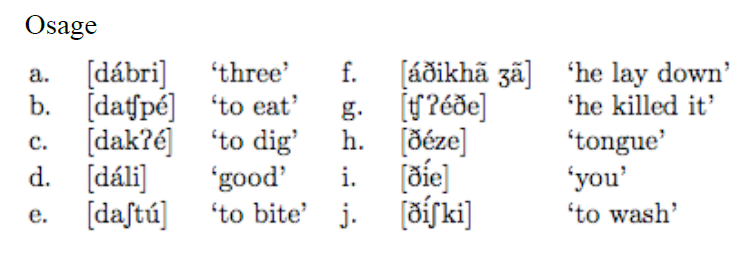
\includegraphics{../images/osage.png}
\end{figure}

~\\
INSTRUCTOR NOTES: is not useful -- there are no alternations in this dataset, so we can't use them to figure out what sounds are relevant to analyse


\vfill
Excellent (3) ~~~ Good (2.2) ~~~ Fair (1.7) ~~~ Poor (0)
\newpage

{\large Question 2}\\

Source: Final Exam Dataset\\

Explain what the underlying representation of these morphemes would be and why.\\

`invent', `progressive'

\begin{figure}[H]
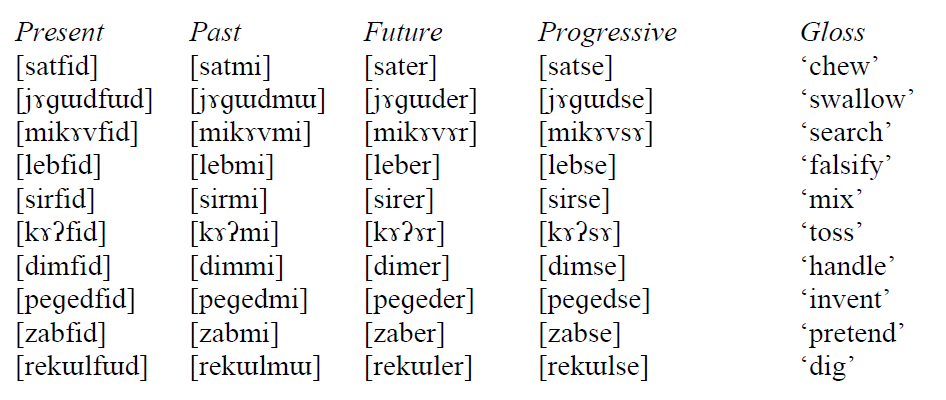
\includegraphics{../images/final_dataset.png}
\end{figure}

~\\
INSTRUCTOR NOTES: For any morpheme that doesn’t alternate, its UR should be the same as its SR.  For the morphemes that alternate, the back-vowel version occurs in the narrower set of contexts (after a back vowel of the same height), so should be the one that we write a rule for. The front-vowel version occurs in the wider / elsewhere set of contexts (after a front vowel and after a back vowel of a different height), so this should be the UR. So in this case, we have the non-alternating root morpheme ‘invent’ /peɡed/ and the alternating suffix morpheme 'progressive' /se/.


\vfill
Excellent (3) ~~~ Good (2.2) ~~~ Fair (1.7) ~~~ Poor (0)
\newpage

{\large Question 3}\\

Source: Day 8 Handout, Question 7\\

Explain why each numbered, underlined statement is true or false. If it is false, explain one way that you could correct it.\\

We can visualize speech through the use of spectra and spectrograms. $^{18}$\ul{A spectrogram shows frequency on the horizontal axis and amplitude on the vertical axis.} $^{19}$\ul{A spectrum, on the other hand, shows frequency on the vertical axis and time along the horizontal axis}.\\\\$^{20}$\ul{On a spectrogram, the dark bars are called formants.} $^{21}$\ul{The formants correspond to the amplitude peaks on a spectrum.}


~\\
INSTRUCTOR NOTES: 18 - false (A spectrum shows frequency on the horizontal axis and amplitude on the vertical axis, or, a spectrogram shows frequency on the vertical axis and time along the horizontal axis).\\19 - false (A spectrum shows frequency on the horizontal axis and amplitude on the vertical axis, or, a spectrogram shows frequency on the vertical axis and time along the horizontal axis).\\20 - true.\\21 - true.


\vfill
Excellent (3) ~~~ Good (2.2) ~~~ Fair (1.7) ~~~ Poor (0)
\newpage

{\large Question 4}\\

Source: Quiz 10, Question 1\\

Section 4.2 of chapter 13 in the Peng textbook presented an autosegmental analysis of Mende tone distribution. Explain why the form shown below should NOT be the UR for any morpheme in Mende.\\

\begin{figure}[H]
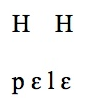
\includegraphics{../images/mende_house_b.png}
\end{figure}

~\\
INSTRUCTOR NOTES: There's no reason to violate the OCP in the UR of a single morpheme, but this one has two adjacent H tones


\vfill
Excellent (3) ~~~ Good (2.2) ~~~ Fair (1.7) ~~~ Poor (0)
\newpage

{\large Question 5}\\

Source: Homework 5, Question 1\\

Explain which sound should be removed to make this a natural class, and what the minimum set of features would be to describe the resulting natural class.\\

{[v]}, {[z]}, {[ʃ]}, {[ʒ]}, {[ð]}


~\\
INSTRUCTOR NOTES: [ʃ] should be removed, so that we have the natural class of voiced fricatives; this could be minimally represented with [+voice, +cont, -son]


\vfill
Excellent (3) ~~~ Good (2.2) ~~~ Fair (1.7) ~~~ Poor (0)
\newpage

{\large Question 6}\\

Source: Quiz 9, Question 12\\

Explain the key differences between the templatic and the rule-based approaches to syllabification.\\


~\\
INSTRUCTOR NOTES: in the rule-based approach, you ONLY have rules, so you don't know ahead of time what possible syllable types you might get; you also need to know which rules apply in a language and what the order of the rules is -- but in the templatic approach, you have a template that tells you ahead of time what the possible syllable types are, and you use the template in conjunction with rules; in the templatic approach, you also need to know the direction of syllabification (L to R or R to L), not the order of the rules [Note: should not mention anything about the units used in either approach)


\vfill
Excellent (3) ~~~ Good (2.2) ~~~ Fair (1.7) ~~~ Poor (0)
\newpage

\begin{center}
\textbf{{\color{red}{\HUGE END OF EXAM}}}\\

\end{center}
\newpage

\begin{center}
\textbf{{\color{blue}{\HUGE START OF EXAM\\}}}

\textbf{{\color{blue}{\HUGE Student ID: 4199\\}}}

\textbf{{\color{blue}{\HUGE 11:50 AM - 12:10 PM\\}}}

\end{center}
\newpage

{\large Question 1}\\

Source: Day 9 Handout, Question 1\\

Explain why the concept of an alternation either is or is not useful for understanding this dataset.\\

\begin{figure}[H]
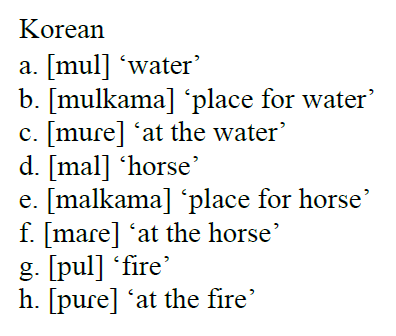
\includegraphics{../images/korean.png}
\end{figure}

~\\
INSTRUCTOR NOTES: is useful -- root morphemes alternate, so we can decide which sounds we need to analyze


\vfill
Excellent (3) ~~~ Good (2.2) ~~~ Fair (1.7) ~~~ Poor (0)
\newpage

{\large Question 2}\\

Source: Day 8 Handout, Question 4\\

Explain how each component of the description below gives you information about the sound being described.\\

This consonant is characterized by having a lot of random noise in the spectrogram, with no clear formant structure at all. It tends to be longer and louder than other similar consonants. There is no voice bar, and the majority of the noise created by this consonant is at relatively high frequencies.


~\\
INSTRUCTOR NOTES: [s]; check for voicing, place, and manner


\vfill
Excellent (3) ~~~ Good (2.2) ~~~ Fair (1.7) ~~~ Poor (0)
\newpage

{\large Question 3}\\

Source: Final Exam Dataset\\

Explain how you would go about figuring out what to analyse in this dataset.\\

\begin{figure}[H]
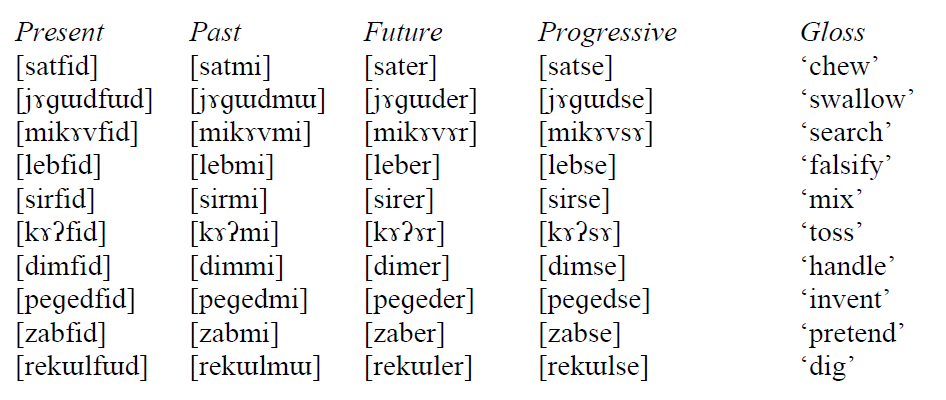
\includegraphics{../images/final_dataset.png}
\end{figure}

~\\
INSTRUCTOR NOTES: The first thing to do is a morphological analysis. There should be morphemes that represent each of the four tenses / aspects (present, past, future, and progressive), and morphemes that represent each root. The morphemes representing the tenses appear as (relatively) consistent forms in the columns; the morphemes representing the roots appear as consistent forms in the rows. Doing this reveals that the final 3 segments in the present forms and the final two segments in the progressive forms are suffixes (there are no zero morphemes, and all components have a one-to-one correspondence). Then we check for alternations. The alternations here are in the suffixes; each of the four suffixes has two forms. There are therefore four alternations, with two allomorphs each. So, what we need to analyze are the alternations in the suffix forms, where we see vowels alternating. Two of the alternations involve [i] and [ɯ], and the other two alternations involve [e] and [ɤ]. In each case, there’s a front vowel and a back vowel, which are otherwise matched for height and rounding, so we can likely generalize across the alternations.


\vfill
Excellent (3) ~~~ Good (2.2) ~~~ Fair (1.7) ~~~ Poor (0)
\newpage

{\large Question 4}\\

Source: Homework 5, Question 1\\

Explain which sound should be removed to make this a natural class, and what the minimum set of features would be to describe the resulting natural class.\\

{[i]}, {[ɪ]}, {[ɛ]}, {[u]}, {[ʊ]}


~\\
INSTRUCTOR NOTES: [ɛ] should be removed, so that we have the natural class of high vowels; this could be minimally represented with [+syll, +high]


\vfill
Excellent (3) ~~~ Good (2.2) ~~~ Fair (1.7) ~~~ Poor (0)
\newpage

{\large Question 5}\\

Source: Day 11 Handout, Question 5\\

Explain why this template either does or does not allow syllables of this type to occur.\\

VCC

\begin{figure}[H]
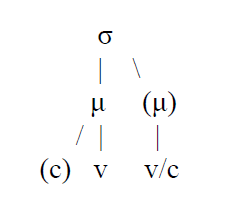
\includegraphics{../images/ponapean_syllabletemplate.png}
\end{figure}

~\\
INSTRUCTOR NOTES: not allowed


\vfill
Excellent (3) ~~~ Good (2.2) ~~~ Fair (1.7) ~~~ Poor (0)
\newpage

{\large Question 6}\\

Source: Day 12 Handout, Question 7\\

Explain how you would figure out the underlying representations of the suffix morphemes in this dataset.\\

\begin{figure}[H]
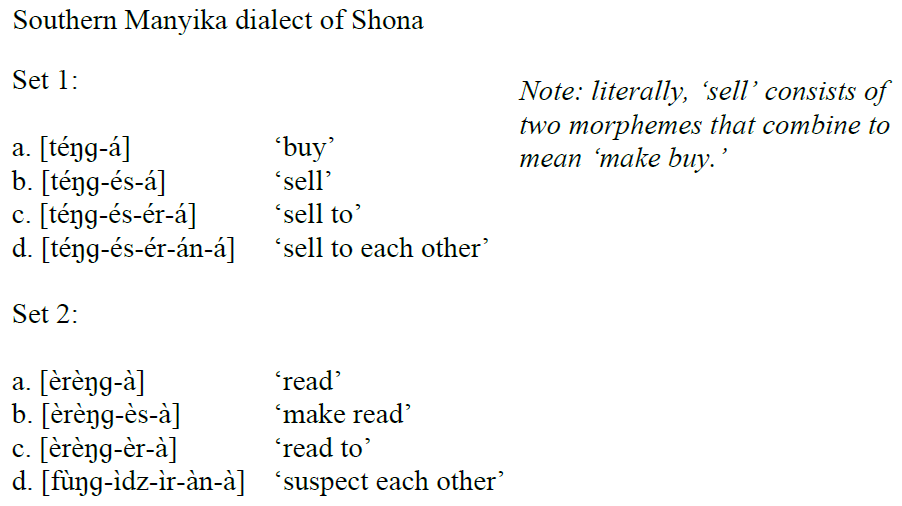
\includegraphics{../images/shona.png}
\end{figure}

~\\
INSTRUCTOR NOTES: the suffix morphemes alternate, so we need to pick either one or the other or something else for their URs; because their tone is always predictable from their context, we can assume that they get the tones just from the tone-mapping procedures and are underlyingly toneless (the segments never alternate, so they are the same as in their URs)


\vfill
Excellent (3) ~~~ Good (2.2) ~~~ Fair (1.7) ~~~ Poor (0)
\newpage

\begin{center}
\textbf{{\color{red}{\HUGE END OF EXAM}}}\\

\end{center}
\newpage

\begin{center}
\textbf{{\color{blue}{\HUGE START OF EXAM\\}}}

\textbf{{\color{blue}{\HUGE Student ID: 1794\\}}}

\textbf{{\color{blue}{\HUGE 12:10 - 12:30 PM\\}}}

\end{center}
\newpage

{\large Question 1}\\

Source: Day 11 Handout, Question 12\\

Explain how understanding syllable structure helps understand the motivation for the process(es) seen in this data.\\

\begin{figure}[H]
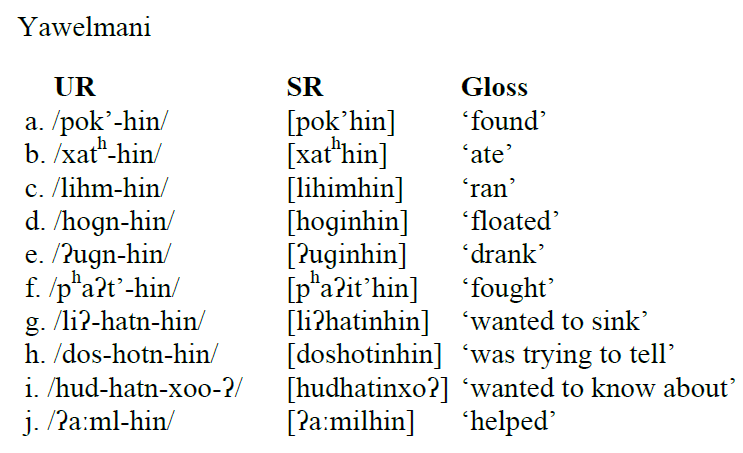
\includegraphics{../images/yawelmani.png}
\end{figure}

~\\
INSTRUCTOR NOTES: although syllabification must happen after insertion, the insertion is motivated by making things syllabifiable -- we insert a vowel into a sequence of CCC in order to prevent any complex onsets / codas or syllabic consonants from having to be used


\vfill
Excellent (3) ~~~ Good (2.2) ~~~ Fair (1.7) ~~~ Poor (0)
\newpage

{\large Question 2}\\

Source: Day 10 Discussion\\

Explain what the given feature’s value is for this class of sounds, and why.\\

{[strident]}

glides


~\\
INSTRUCTOR NOTES: 0, because [strident] applies only to obstruents, and glides are sonorants


\vfill
Excellent (3) ~~~ Good (2.2) ~~~ Fair (1.7) ~~~ Poor (0)
\newpage

{\large Question 3}\\

Source: Final Exam Dataset\\

Explain what the underlying representation of these morphemes would be and why.\\

`mix', `past'

\begin{figure}[H]
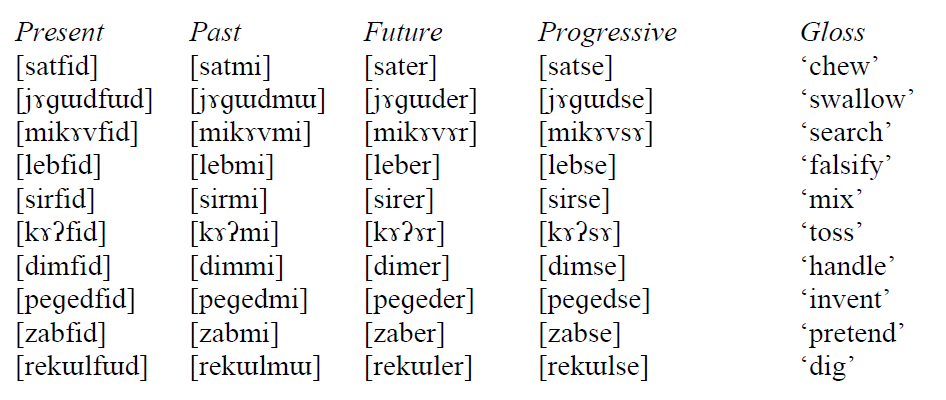
\includegraphics{../images/final_dataset.png}
\end{figure}

~\\
INSTRUCTOR NOTES: For any morpheme that doesn’t alternate, its UR should be the same as its SR.  For the morphemes that alternate, the back-vowel version occurs in the narrower set of contexts (after a back vowel of the same height), so should be the one that we write a rule for. The front-vowel version occurs in the wider / elsewhere set of contexts (after a front vowel and after a back vowel of a different height), so this should be the UR. So in this case, we have the non-alternating root morpheme ‘mix’ /sir/ and the alternating suffix morpheme 'past' /mi/.


\vfill
Excellent (3) ~~~ Good (2.2) ~~~ Fair (1.7) ~~~ Poor (0)
\newpage

{\large Question 4}\\

Source: Day 12 Handout, Question 5\\

Explain which of the three rules will apply to the form given below, and whether each of those rules would have an effect or not.\\

Peng’s Tone-Mapping Procedure for Mende: \begin{enumerate} \item L-to-R association: Associate the first tone to the first TBU, the second tone to the second TBU, and so on, until all tones or all TBUS are exhausted. \item Last-TBU Linking: Associate any remaining unlinked tones to the last TBU. \item Last-Tone Linking: Associate the last tone to any TBU without a tone. \end{enumerate}

\begin{figure}[H]
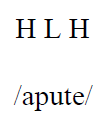
\includegraphics{../images/mendetone_a.png}
\end{figure}

~\\
INSTRUCTOR NOTES: L-to-R association is the only one that applies; it links up each of the three tones to a TBU, and then the other rules have nothing to do, because their context isn't met (there are no leftover tones or TBUs)


\vfill
Excellent (3) ~~~ Good (2.2) ~~~ Fair (1.7) ~~~ Poor (0)
\newpage

{\large Question 5}\\

Source: Day 9 Handout, Question 5\\

Explain which morpheme(s) in this dataset alternate and how that helps you do a phonological analysis.\\

\begin{figure}[H]
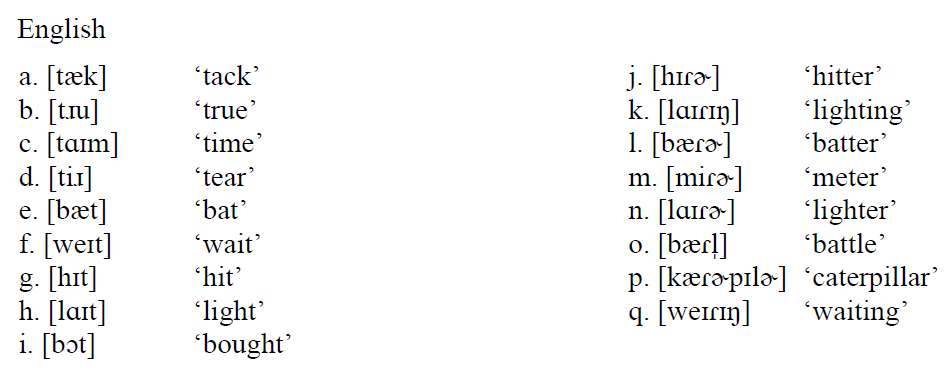
\includegraphics{../images/english_t_flap.png}
\end{figure}

~\\
INSTRUCTOR NOTES: some of the roots alternate (such as 'light'), so we know that we need to analyze the predictable occurrence of [t] vs. [flap]


\vfill
Excellent (3) ~~~ Good (2.2) ~~~ Fair (1.7) ~~~ Poor (0)
\newpage

{\large Question 6}\\

Source: Day 8 Handout, Question 3\\

Explain what you see in the spectrogram that tells you about the properties of the sounds in the pictured word.\\

\begin{figure}[H]
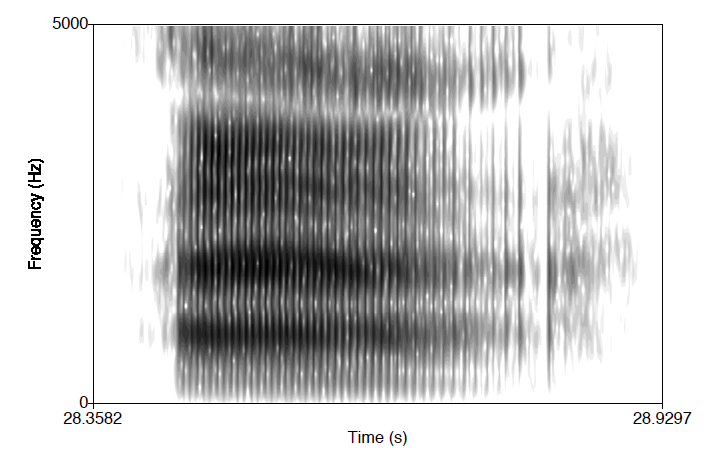
\includegraphics{../images/spectrogram_aaah.png}
\end{figure}

~\\
INSTRUCTOR NOTES: aaah: just a vowel; formants are very steady; F1 and F2 are pretty close to each other; F1 somewhat high and F2 somewhat low


\vfill
Excellent (3) ~~~ Good (2.2) ~~~ Fair (1.7) ~~~ Poor (0)
\newpage

\begin{center}
\textbf{{\color{red}{\HUGE END OF EXAM}}}\\

\end{center}
\newpage

\begin{center}
\textbf{{\color{blue}{\HUGE START OF EXAM\\}}}

\textbf{{\color{blue}{\HUGE Student ID: 4656\\}}}

\textbf{{\color{blue}{\HUGE 12:30 - 12:50 PM\\}}}

\end{center}
\newpage

{\large Question 1}\\

Source: Day 11 Handout, Question 10\\

Explain why this structure either is or is not a correct application of the templatic-based approach to syllabification, using the provided template and assuming that syllabification proceeds from left to right.\\

\begin{figure}[H]
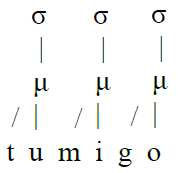
\includegraphics{../images/pengtemplate_tumigo_yes.png}
\end{figure}
\begin{figure}[H]
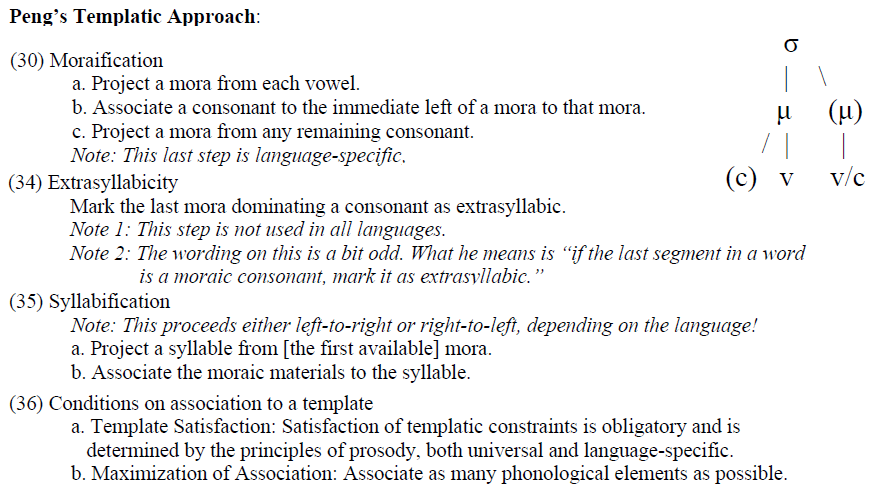
\includegraphics{../images/peng_template_withdiagram.png}
\end{figure}

~\\
INSTRUCTOR NOTES: yes; this is just all CV syllables


\vfill
Excellent (3) ~~~ Good (2.2) ~~~ Fair (1.7) ~~~ Poor (0)
\newpage

{\large Question 2}\\

Source: Day 10 Handout, Question 5\\

Explain why you either should or should not use phonological features in the CONTEXT of the given rule.\\

Vowel laxing: /i/ → {[ɪ]} / \{{[ɛ]}, {[ɔ]}\} C$_0$\_\_


~\\
INSTRUCTOR NOTES: yes; you're trying to group multiple (in this case, two) sounds together, so it's good to use features to describe their commonality; it also helps us see the naturalness of the rule by pointing out the relevant part of the phonological context


\vfill
Excellent (3) ~~~ Good (2.2) ~~~ Fair (1.7) ~~~ Poor (0)
\newpage

{\large Question 3}\\

Source: Final Exam Dataset\\

Explain how you would go about figuring out what to analyse in this dataset.\\

\begin{figure}[H]
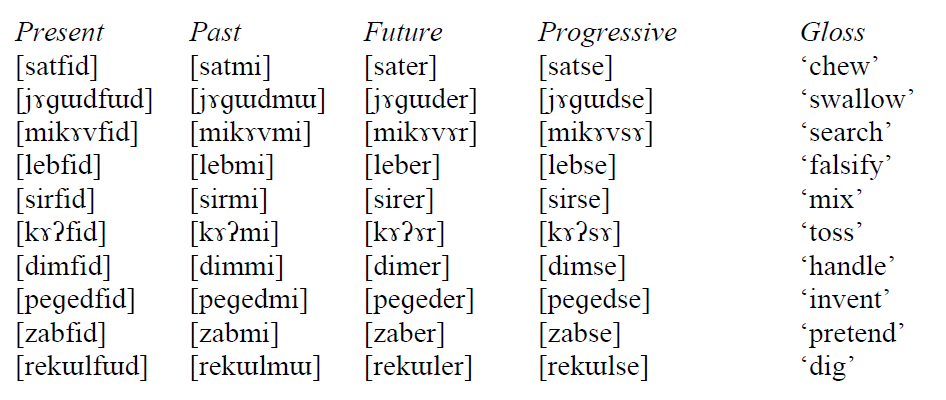
\includegraphics{../images/final_dataset.png}
\end{figure}

~\\
INSTRUCTOR NOTES: The first thing to do is a morphological analysis. There should be morphemes that represent each of the four tenses / aspects (present, past, future, and progressive), and morphemes that represent each root. The morphemes representing the tenses appear as (relatively) consistent forms in the columns; the morphemes representing the roots appear as consistent forms in the rows. Doing this reveals that the final 3 segments in the present forms and the final two segments in the progressive forms are suffixes (there are no zero morphemes, and all components have a one-to-one correspondence). Then we check for alternations. The alternations here are in the suffixes; each of the four suffixes has two forms. There are therefore four alternations, with two allomorphs each. So, what we need to analyze are the alternations in the suffix forms, where we see vowels alternating. Two of the alternations involve [i] and [ɯ], and the other two alternations involve [e] and [ɤ]. In each case, there’s a front vowel and a back vowel, which are otherwise matched for height and rounding, so we can likely generalize across the alternations.


\vfill
Excellent (3) ~~~ Good (2.2) ~~~ Fair (1.7) ~~~ Poor (0)
\newpage

{\large Question 4}\\

Source: Quiz 7, Question 8\\

Based on this data from Lamba, explain why the pair given below either does or does not show that the consonants preceding the morpheme for `with' are NOT responsible for the variation between [-il] and [-el].\\

tul-il-a \& soŋk-el-a

\begin{figure}[H]
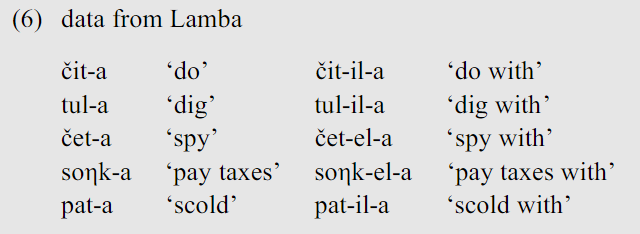
\includegraphics{../images/peng119_lamba.png}
\end{figure}

~\\
INSTRUCTOR NOTES: doesn't show this -- we do see [il] and [el], but they occur after different consonants, so it COULD be the consonant that is responsible


\vfill
Excellent (3) ~~~ Good (2.2) ~~~ Fair (1.7) ~~~ Poor (0)
\newpage

{\large Question 5}\\

Source: Day 8 Handout, Question 3\\

Explain what you see in the spectrogram that tells you about the properties of the sounds in the pictured word.\\

\begin{figure}[H]
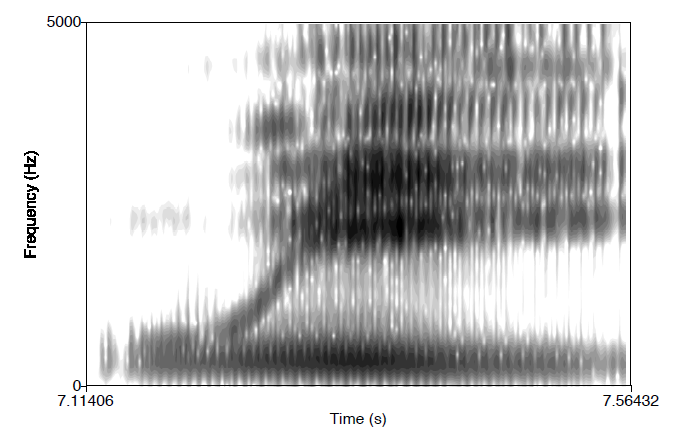
\includegraphics{../images/spectrogram_we.png}
\end{figure}

~\\
INSTRUCTOR NOTES: we: starts paler, then darker, so glide plus vowel; F1 pretty constantly low (=high V); F2 starts very low and then swoops up (=starts back and goes front)


\vfill
Excellent (3) ~~~ Good (2.2) ~~~ Fair (1.7) ~~~ Poor (0)
\newpage

{\large Question 6}\\

Source: Day 12 Handout, Question 5\\

Explain which of the three rules will apply to the form given below, and whether each of those rules would have an effect or not.\\

Peng’s Tone-Mapping Procedure for Mende: \begin{enumerate} \item L-to-R association: Associate the first tone to the first TBU, the second tone to the second TBU, and so on, until all tones or all TBUS are exhausted. \item Last-TBU Linking: Associate any remaining unlinked tones to the last TBU. \item Last-Tone Linking: Associate the last tone to any TBU without a tone. \end{enumerate}

\begin{figure}[H]
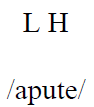
\includegraphics{../images/mendetone_c.png}
\end{figure}

~\\
INSTRUCTOR NOTES: L-to-R association applies and links the H tone to the first TBU [a] and the L tone to the second TBU [u]; last-TBU linking doesn't apply because there are no leftover tones; then last-tone linking does apply, and connects all of the leftover TBUs (in this case, [e]) to the final tone (in this case, L)


\vfill
Excellent (3) ~~~ Good (2.2) ~~~ Fair (1.7) ~~~ Poor (0)
\newpage

\begin{center}
\textbf{{\color{red}{\HUGE END OF EXAM}}}\\

\end{center}
\newpage

\begin{center}
\textbf{{\color{blue}{\HUGE START OF EXAM\\}}}

\textbf{{\color{blue}{\HUGE Student ID: 8079\\}}}

\textbf{{\color{blue}{\HUGE 12:50 - 1:10 PM\\}}}

\end{center}
\newpage

{\large Question 1}\\

Source: Day 8 Handout, Question 1\\

Explain what (if anything) the letter below represents on this waveform.\\

C

\begin{figure}[H]
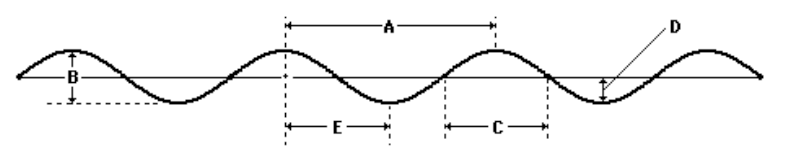
\includegraphics{../images/sinusoid.png}
\end{figure}

~\\
INSTRUCTOR NOTES: nothing (half wavelength or half period)


\vfill
Excellent (3) ~~~ Good (2.2) ~~~ Fair (1.7) ~~~ Poor (0)
\newpage

{\large Question 2}\\

Source: Quiz 8, Question 3\\

Explain why this featural specification either does or does not match the given sound.\\

{[-consonantal]}, {[-sonorant]}

{[u]}


~\\
INSTRUCTOR NOTES: does not match: [u] is [-cons], but is [+son]


\vfill
Excellent (3) ~~~ Good (2.2) ~~~ Fair (1.7) ~~~ Poor (0)
\newpage

{\large Question 3}\\

Source: Final Exam Dataset\\

Explain what rule or rules would apply in this dataset and how you know.\\

\begin{figure}[H]
\includegraphics{../images/final_dataset.png}
\end{figure}

~\\
INSTRUCTOR NOTES: We need a rule of "Vowel Backing" as follows: [α high, +syllabic] --> [+back] / [α high, +back, +syllabic] C0 \_\_. This rule says that a vowel will become back if it follows another back vowel of the same height, regardless of any intervening consonants. We know this is the rule we need because we need to account for the suffix alternations; the suffixes appear either with a front vowel or a back vowel. The back versions occur only after a back vowel of the same height (so are the focus of the rule); the front vowels occur elsewhere (after a front vowel, or after a back vowel of a different height). We could have two separate rules, one for mid vowels and one for high vowels, but this misses the generalization that these rules are basically doing the same thing.


\vfill
Excellent (3) ~~~ Good (2.2) ~~~ Fair (1.7) ~~~ Poor (0)
\newpage

{\large Question 4}\\

Source: Day 9 Handout, Question 3\\

Explain which morpheme(s) in this dataset alternate and how that helps you do a phonological analysis.\\

\begin{figure}[H]
\includegraphics{../images/english_past.png}
\end{figure}

~\\
INSTRUCTOR NOTES: the past tense morpheme alternates, so we know we need to analyze the predictable occurrence of [t] vs. [d]


\vfill
Excellent (3) ~~~ Good (2.2) ~~~ Fair (1.7) ~~~ Poor (0)
\newpage

{\large Question 5}\\

Source: Day 12 Handout, Question 6\\

Explain how you would figure out the tone-mapping procedures that apply in this dataset.\\

\begin{figure}[H]
\includegraphics{../images/kukuya.png}
\end{figure}

~\\
INSTRUCTOR NOTES: You probably start with procedures that you know work for some other language like Mende, and see whether they work here. In this case, we (1) look at cases of words that have one of the contour tones, because words with only H or only L will just always have a single tone associated with all of the TBUs, but contour tones can help you see e.g. “where” the contour happens; (2) look at cases of words with a mismatch in the number of tones and TBUs (e.g. HL tones and VVV, or LHL tones and VV), because these are cases where one-to-one mapping will fail. By seeing that the “tail” of contours is to the left, not the right (e.g., it’s LLH not LHH) and that in the triple-tone words with two TBUs, we have the contour to the left (LH, then L; not L, then HL), we see that the “leftover” stuff needs to be on the left edge instead of the right edge. Hence, the initial mapping procedure should proceed from right to left instead of left to right.


\vfill
Excellent (3) ~~~ Good (2.2) ~~~ Fair (1.7) ~~~ Poor (0)
\newpage

{\large Question 6}\\

Source: Homework 5, Question 2\\

Explain why the insertion analysis is better than the deletion analysis for this dataset.\\

\begin{figure}[H]
\includegraphics{../images/fula.png}
\end{figure}

~\\
INSTRUCTOR NOTES: If you have /VC/ as the underlying form of these suffixes, there’s no reason to delete the vowel, because you'd have perfect CV syllables throughout the word. But if you have /C/ as the underlying form, it’s clear that we occasionally need an extra vowel in order to allow syllabification to happen; otherwise, we’d end up with non-syllabifiable CCC sequences. That is, there’s a phonological motivation for the insertion rule, but no motivation for the deletion rule.


\vfill
Excellent (3) ~~~ Good (2.2) ~~~ Fair (1.7) ~~~ Poor (0)
\newpage

\begin{center}
\textbf{{\color{red}{\HUGE END OF EXAM}}}\\

\end{center}
\newpage

\end{document}

